\subsection{Raster datamodel} \label{Afsnit: Raster data model}

En rastermodel er en datamodel der er bygget op af et regulært netværk af celler organiseret i et gitterformat \citep{bolstad_gis_2022, esri_raster}. Hver celle i en raster model er karakteriseret af en celle dimension, som definerer cellestørrelsen ud fra cellens længde i X- og Y-retningen \citep{bolstad_gis_2022}. Cellestørrelsen repræsenterer således den rumlige opløsning af raster datamodellen og fungerer som en indikator for den rumlige præcision, da hver celles koordinat er givet ud fra centrum af cellen. En større cellestørrelse vil derfor resultere i en højere rumlig usikkerhed, mens en mindre cellestørrelse vil medføre en lavere rumlig usikkerhed. En større cellestørrelse medfører også et større datasæt og optager mere plads i databaser \citep{bolstad_gis_2022}. Rastermodellen er derfor en afvejning af opløsning og filstørrelse.\\

Hver cele i en raster indeholder en værdi, der repræsenterer information om det pågældende geografiske område. Disse værdier kan enten være numeriske eller kategoriske, afhængigt af den type data, der ønskes repræsenteret. Numeriske værdier anvendes typisk til at beskrive kontinuerlige data, hvor værdierne kan variere gradvist fra celle til celle. Et eksempel på dette er højdemodeller, hvor hver celle indeholder en talværdi, der angiver terrænets højde (figur \ref{Subfig: Kontinuer raster}). Andre eksempler på kontinuerlige rasterdata er temperatur, nedbør eller koncentration af et bestemt stof i jorden. \\
Kategoriske værdier bruges derimod til at repræsentere diskrete eller tematiske vædier, hvor hver celle tildeles en bestemt kategori eller klasse. Dette ses fx i arealanvendelseskort, hvor hver celle angiver om området er dækket af skov eller trætyper (figur \ref{Subfig: Kategorisk raster}).
\begin{figure}[H]
    \begin{subfigure} [t]{0.5\textwidth}
        \centering
        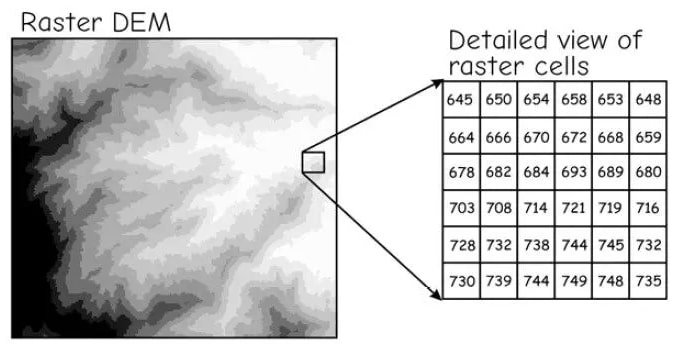
\includegraphics[width=1\linewidth]{images/teori/raster_kontinuert.jpg}
        \caption{}
        \label{Subfig: Kontinuer raster}
    \end{subfigure}
    \begin{subfigure} [t]{0.5\textwidth}
        \centering
        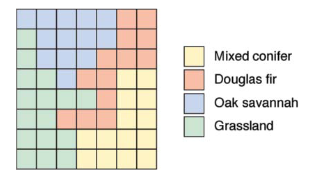
\includegraphics[width=1\linewidth]{images/teori/raster_areal.png}
        \caption{}
        \label{Subfig: Kategorisk raster}
    \end{subfigure}
    \caption{Eksempel på en raster med numeriske kontinuert data fra en højdemodel \textbf{(a)} og en kategorisk raster med diskrete data over forskellige trætyper og arealanvendelser\textbf{(b)}. Kilde: \cite[s. 66]{bolstad_gis_2022} og \cite[s. 67]{longley_geographical_2008}}
    \label{Figur: Kontinuert og kategorisk raster}
\end{figure}
Det er vigtigt at bemærke at rasterceller også kan indeholde en unik værdi, der angiver 'NoData', hvis der ikke foreligger information for det pågældende område. NoData værdier gør det muligt at håndtere ufuldstændige datasæt og sikring at analyser kun udføres på relevante celler \citep{bolstad_gis_2022, longley_geographical_2008}.

Rastermodellens struktur muliggør omfattende rumlig analyse, idet der kan udføres artimetiske og logiske operationer på tværs af celler og mellem flere forskellige typer af rasterlag. Denne egenskab gør det derfor muligt at analysere og kombinere kontinuerte og diskrete rumlige informationer i et GIS-miljø  \citep{bolstad_gis_2022, longley_geographical_2008}. Det er også muligt at udføre analyse mellem raster og vektordata. Ved at udføre analyse med begge datatyper er det muligt at lave kombineret vektor- og raster modeller i et GIS-miljø der blandt andet kan bruges til at lave stormflodsmodellering.

\subsection{Inundation Modellen} \label{Afsnit: Inundation Model}

Til projektet er der blevet anvendt en GIS-baseret stormflods model kaldet \textit{"Inundation Model"} udarbejdet af \cite{balstrom_kirby_inundation} til at give et bud på hvordan en stormflod vil påvirke et område. Modellen opererer eksklusivt i et ArcGIS Pro miljø, GIS-softwaren udviklet af Esri.\\
Modellen indeholder en række værktøjer, der bruges til at analysere stormfloders påvirkning af et område og kernen i modellen er værktøjet \textit{"Create Inundation"}, en statisk numerisk rastermodel. Modellen tager tre brugerdefineret parametre der består af tre numeriske værdier i meter som input: InitialSealLevel, SeaLevelIncrement og Number of Iterations. InitialSeaLevel bruges som en startværdi for modellen til at itererer over. SeaLevelIncrement er den værdi modellen skal stige med efter hver iteration (fx 1 cm stigning). Number of Iterations er antallet af gentagelser modellen udører. \\
Modellen benytter en hydrologisk korrigeret Digital Terræn Model (DHyM) og et digitaliseret linjeobjekt som kilde for udregningen, benævt Line at Sea \citep{balstrom_kirby_inundation}. I figur \ref{Figur: Create Inundation} er modellens struktur vist inddelt i to segmenter.
\begin{figure}[H]
    \centering
    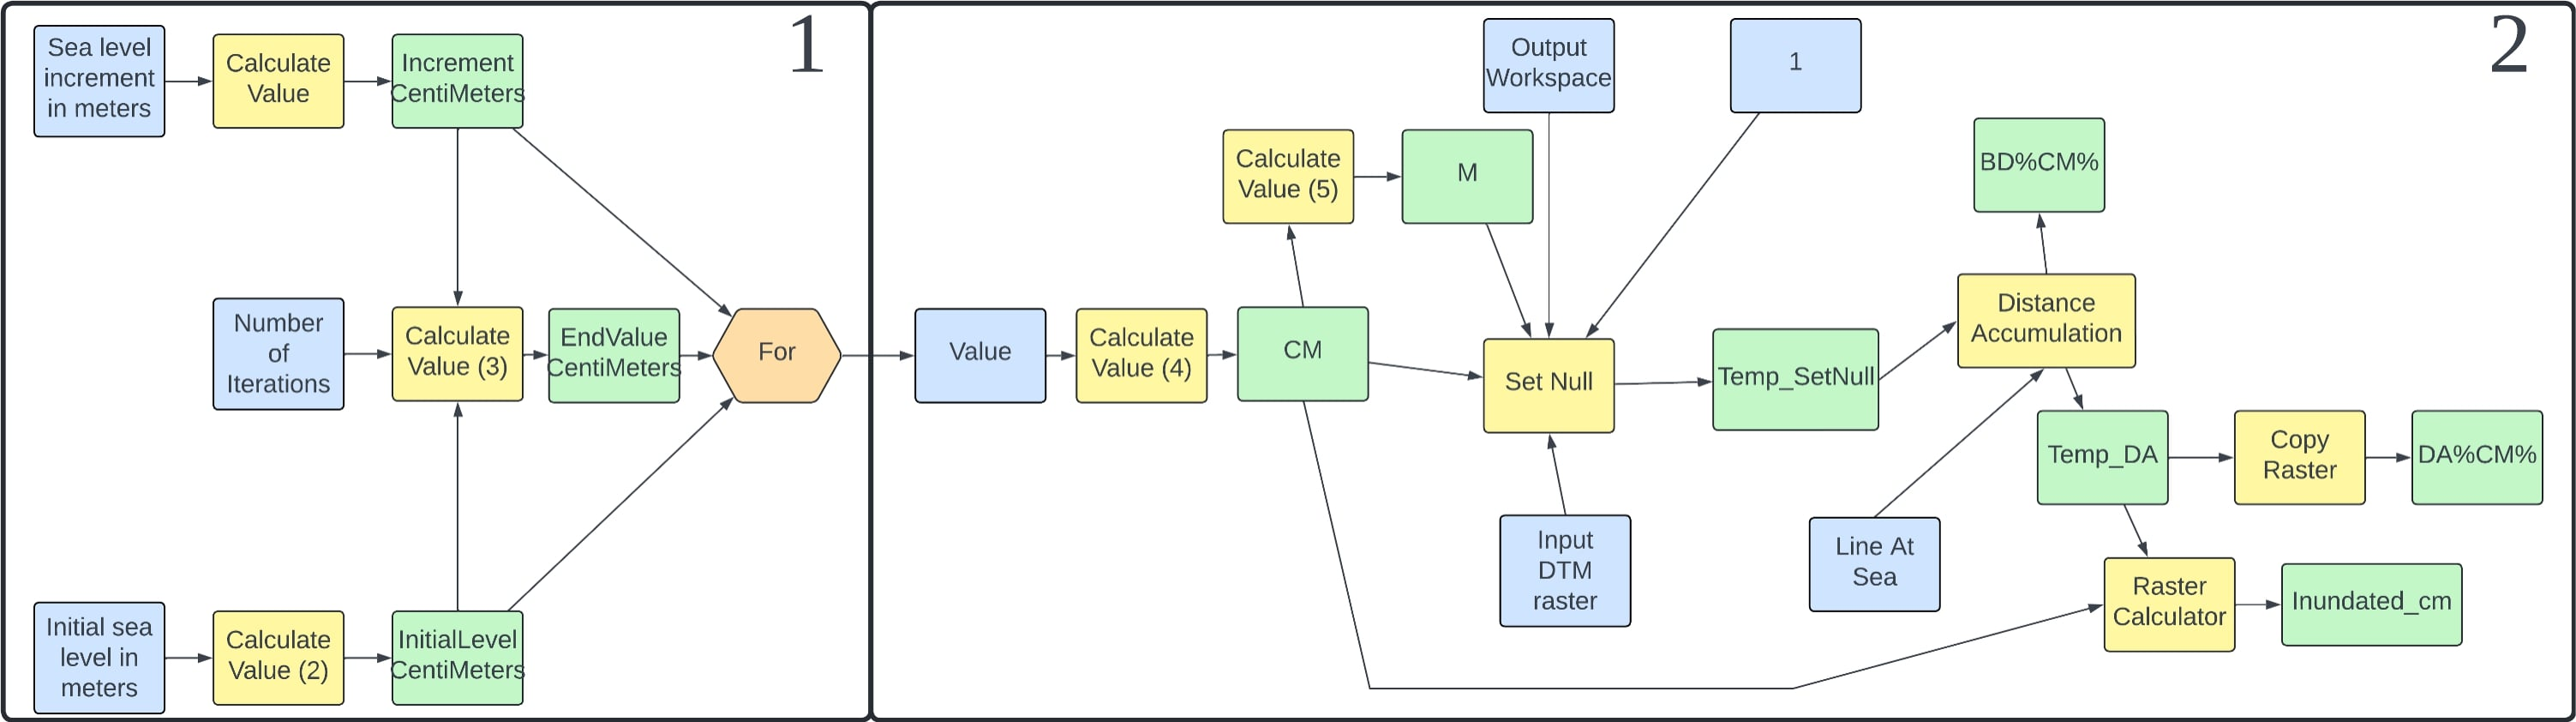
\includegraphics[width=1\linewidth]{images/teori/inundation_model_separated.jpg}
    \caption{Flowchart af Inundation Modellens \textit{"Create Inundation"} værktøj.}
    \label{Figur: Create Inundation}
\end{figure}


Det første segment er en omregning af brugerens input fra meter til centimeter for både stigningsniveauet for hver gang modellen itererer og det begyndende havniveau. Modellen kræver en afsluttende værdi for hvornår den skal stoppe med at iterere, som svarer til den vandstand der ønskes at simulere op til. Denne værdi bliver udregnet ved følgende: \\$InitialSeaLevel + ((NumberIterations - 1)\times Increment)$. På samme vis kan en omvendt udregning laves for at finde antallet af gentagelser for at opnå en bestemt vandstand. Dette gøres ved: $(EndValue - InitialSeaLevel) / Increment - 1$. Dette tillader brugeren at simulere til en ønsket vandstand.\\

Det andet segment af modellen er selve oversvømmelses beregningen gennem højdemodellen. Det starter med et for-loop der starter med den første værdi (fx 100 cm). Denne værdi omregnes tilbage til meter hvorefter modellen eksekverer et hvis-ellers tjek (figur \ref{Figur: Create Inundation} "SetNull") på cellerne i DTM. Her tjekkes alle celleværdierne i DTM for om de er større eller ligmed den pågældende værdi. Hvis dette hvis-ellers tjek er sandt når værdien i DTM er højere end tjekværdi, bliver cellerne tildelt NoData værdien, som indikerer at cellen ikke bliver oversvømmet ved dette oversvømmelsesniveau. Hvis DTM celleværdien er lavere end tjekværdien og udtrykket dermed er falsk bliver cellen angivet med et 1, som indikerer at cellen oversvømmes ved det niveau. I figur \ref{Figur: Celler Inundated} er der vist hvordan det sker for tre iterationer startende på 100 cm med en stigning på 10 cm. Her det værd at nævne at hver celle der tjekkes for ikke udelukker hinanden, så den næste værdi (110 cm) vil også tildele et 1 til de samme celler, som den foregående værdi.       
\begin{figure}[H]
    \centering
    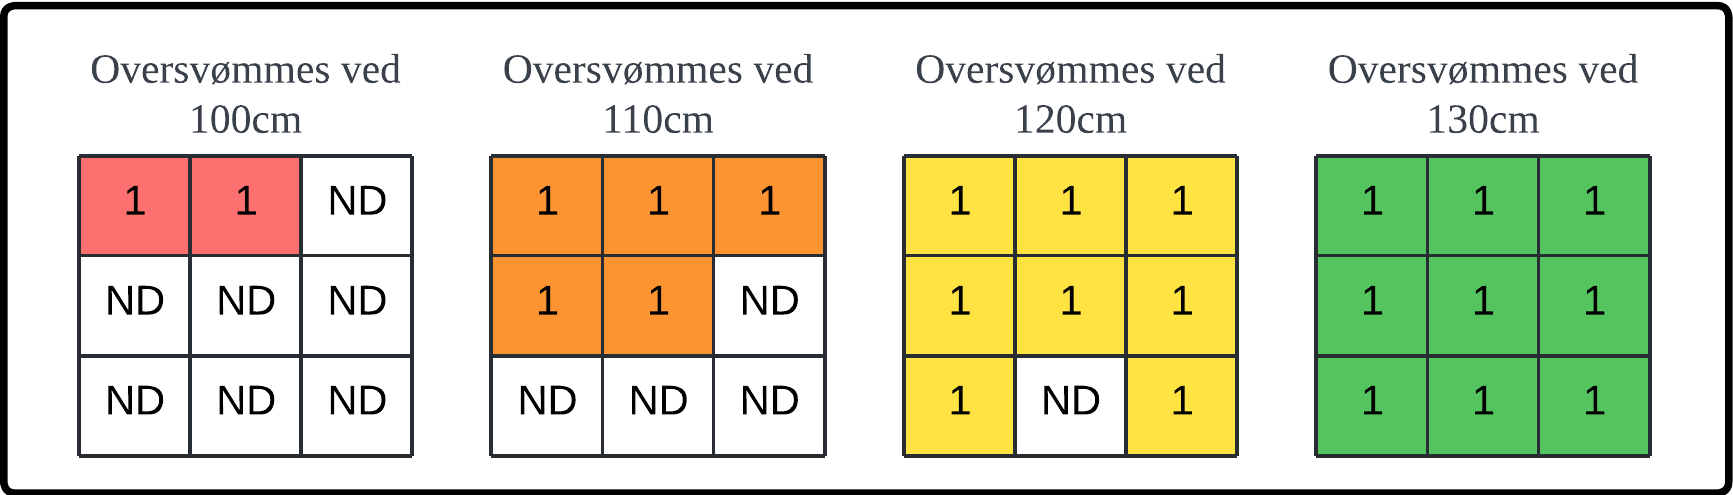
\includegraphics[width=0.7\linewidth]{images/teori/celler_inundated.png}
    \caption{Princippet bag Inundation Modellen gennem cellerne i en højdemodel. 1 angiver at cellen oversvømmes ved det pågældende niveau og ND = NoData (celler som ikke bliver oversvømmet). Egen illustration med inspiration fra \cite{balstrom_kirby_inundation}.}
    \label{Figur: Celler Inundated}
\end{figure}
Herefter gennemføres en Distance Accumulation-analyse igennem de celler der bliver oversvømmet ved det bestemte niveau fra linjekilden Line at Sea. En Distance Accumulation er en analysemetode der beregner den samlede afstand fra en defineret kilde ud igennem et område \citep{esri_how_nodate}. I Inundation modellen bliver Distance Accumulation brugt til at efterligne vandets bevægelse igennem cellerne på samme måde som vandet ville sprede sig under en stormflod. Distance Accumulation forsætter gennem terrænet, indtil der mødes en uigennemtrængelig barriere. Til at sprede sig igennem terrænet bruges der en "eight-side" \hspace{0.2cm}regel, der er med til at bestemme hvilke celler der kan spredes til. Eight-side reglen fortæller Distance Accumulation værktøjet at der skal tjekkes for en passerbar celle i otte retninger fra en celle.\\

I Inundation Modellen starter Distance Accumulation fra linjen \textit{"Line at Sea"} og bevæger sig igennem alle cellerne i terrænet hvor cellen = 1. Hvis cellen er NoData så kan vandet ikke bevæge sig igennem \citep{balstrom_kirby_inundation}. Resultatet af Distance Accumulationen bliver derefter koblet med det oversvømmelsesniveau der bliver itereret over for at give resultatet af modellen og processen starter derefter forfra indtil slutværdien gennemføres.  
